\documentclass{ximera}


%\usepackage{todonotes}

\newcommand{\todo}{}

\usepackage{tkz-euclide}
\tikzset{>=stealth} %% cool arrow head
\tikzset{shorten <>/.style={ shorten >=#1, shorten <=#1 } } %% allows shorter vectors

\usepackage{tkz-tab}  %% sign charts
\usetikzlibrary{decorations.pathreplacing} 

\usetikzlibrary{backgrounds} %% for boxes around graphs
\usetikzlibrary{shapes,positioning}  %% Clouds and stars
\usetikzlibrary{matrix} %% for matrix
\usepgfplotslibrary{polar} %% for polar plots
\usetkzobj{all}
\usepackage[makeroom]{cancel} %% for strike outs
%\usepackage{mathtools} %% for pretty underbrace % Breaks Ximera
\usepackage{multicol}

\usepackage{polynom}



\usepackage[many]{tcolorbox}  %% for titled boxes
\newtcolorbox{xbox}[1]{%
    tikznode boxed title,
    enhanced,
    arc=0mm,
    interior style={white},
    attach boxed title to top center= {yshift=-\tcboxedtitleheight/2},
    fonttitle=\bfseries,
    colbacktitle=white,coltitle=black,
    boxed title style={size=normal,colframe=white,boxrule=0pt},
    title={#1}}


\usepackage{array}
\setlength{\extrarowheight}{+.1cm}   
\newdimen\digitwidth
\settowidth\digitwidth{9}
\def\divrule#1#2{
\noalign{\moveright#1\digitwidth
\vbox{\hrule width#2\digitwidth}}}





\newcommand{\RR}{\mathbb R}
\newcommand{\R}{\mathbb R}
\newcommand{\N}{\mathbb N}
\newcommand{\Z}{\mathbb Z}

%\renewcommand{\d}{\,d\!}
\renewcommand{\d}{\mathop{}\!d}
\newcommand{\dd}[2][]{\frac{\d #1}{\d #2}}
\newcommand{\pp}[2][]{\frac{\partial #1}{\partial #2}}
\renewcommand{\l}{\ell}
\newcommand{\ddx}{\frac{d}{\d x}}
\newcommand{\ddt}{\frac{d}{\d t}}

\newcommand{\zeroOverZero}{\ensuremath{\boldsymbol{\tfrac{0}{0}}}}
\newcommand{\inftyOverInfty}{\ensuremath{\boldsymbol{\tfrac{\infty}{\infty}}}}
\newcommand{\zeroOverInfty}{\ensuremath{\boldsymbol{\tfrac{0}{\infty}}}}
\newcommand{\zeroTimesInfty}{\ensuremath{\small\boldsymbol{0\cdot \infty}}}
\newcommand{\inftyMinusInfty}{\ensuremath{\small\boldsymbol{\infty - \infty}}}
\newcommand{\oneToInfty}{\ensuremath{\boldsymbol{1^\infty}}}
\newcommand{\zeroToZero}{\ensuremath{\boldsymbol{0^0}}}
\newcommand{\inftyToZero}{\ensuremath{\boldsymbol{\infty^0}}}



\newcommand{\numOverZero}{\ensuremath{\boldsymbol{\tfrac{\#}{0}}}}
\newcommand{\dfn}{\textbf}
%\newcommand{\unit}{\,\mathrm}
\newcommand{\unit}{\mathop{}\!\mathrm}
\newcommand{\eval}[1]{\bigg[ #1 \bigg]}
\newcommand{\seq}[1]{\left( #1 \right)}
\renewcommand{\epsilon}{\varepsilon}
\renewcommand{\iff}{\Leftrightarrow}

\DeclareMathOperator{\arccot}{arccot}
\DeclareMathOperator{\arcsec}{arcsec}
\DeclareMathOperator{\arccsc}{arccsc}
\DeclareMathOperator{\si}{Si}
\DeclareMathOperator{\proj}{proj}
\DeclareMathOperator{\scal}{scal}


\newcommand{\tightoverset}[2]{% for arrow vec
  \mathop{#2}\limits^{\vbox to -.5ex{\kern-0.75ex\hbox{$#1$}\vss}}}
\newcommand{\arrowvec}[1]{\tightoverset{\scriptstyle\rightharpoonup}{#1}}
\renewcommand{\vec}{\mathbf}
\newcommand{\veci}{\vec{i}}
\newcommand{\vecj}{\vec{j}}
\newcommand{\veck}{\vec{k}}
\newcommand{\vecl}{\boldsymbol{\l}}

\newcommand{\dotp}{\bullet}
\newcommand{\cross}{\boldsymbol\times}
\newcommand{\grad}{\boldsymbol\nabla}
\newcommand{\divergence}{\grad\dotp}
\newcommand{\curl}{\grad\cross}
%\DeclareMathOperator{\divergence}{divergence}
%\DeclareMathOperator{\curl}[1]{\grad\cross #1}


\colorlet{textColor}{black} 
\colorlet{background}{white}
\colorlet{penColor}{blue!50!black} % Color of a curve in a plot
\colorlet{penColor2}{red!50!black}% Color of a curve in a plot
\colorlet{penColor3}{red!50!blue} % Color of a curve in a plot
\colorlet{penColor4}{green!50!black} % Color of a curve in a plot
\colorlet{penColor5}{orange!80!black} % Color of a curve in a plot
\colorlet{fill1}{penColor!20} % Color of fill in a plot
\colorlet{fill2}{penColor2!20} % Color of fill in a plot
\colorlet{fillp}{fill1} % Color of positive area
\colorlet{filln}{penColor2!20} % Color of negative area
\colorlet{fill3}{penColor3!20} % Fill
\colorlet{fill4}{penColor4!20} % Fill
\colorlet{fill5}{penColor5!20} % Fill
\colorlet{gridColor}{gray!50} % Color of grid in a plot

\newcommand{\surfaceColor}{violet}
\newcommand{\surfaceColorTwo}{redyellow}
\newcommand{\sliceColor}{greenyellow}




\pgfmathdeclarefunction{gauss}{2}{% gives gaussian
  \pgfmathparse{1/(#2*sqrt(2*pi))*exp(-((x-#1)^2)/(2*#2^2))}%
}


%%%%%%%%%%%%%
%% Vectors
%%%%%%%%%%%%%

%% Simple horiz vectors
\renewcommand{\vector}[1]{\left\langle #1\right\rangle}


%% %% Complex Horiz Vectors with angle brackets
%% \makeatletter
%% \renewcommand{\vector}[2][ , ]{\left\langle%
%%   \def\nextitem{\def\nextitem{#1}}%
%%   \@for \el:=#2\do{\nextitem\el}\right\rangle%
%% }
%% \makeatother

%% %% Vertical Vectors
%% \def\vector#1{\begin{bmatrix}\vecListA#1,,\end{bmatrix}}
%% \def\vecListA#1,{\if,#1,\else #1\cr \expandafter \vecListA \fi}

%%%%%%%%%%%%%
%% End of vectors
%%%%%%%%%%%%%

%\newcommand{\fullwidth}{}
%\newcommand{\normalwidth}{}



%% makes a snazzy t-chart for evaluating functions
%\newenvironment{tchart}{\rowcolors{2}{}{background!90!textColor}\array}{\endarray}

%%This is to help with formatting on future title pages.
\newenvironment{sectionOutcomes}{}{} 



%% Flowchart stuff
%\tikzstyle{startstop} = [rectangle, rounded corners, minimum width=3cm, minimum height=1cm,text centered, draw=black]
%\tikzstyle{question} = [rectangle, minimum width=3cm, minimum height=1cm, text centered, draw=black]
%\tikzstyle{decision} = [trapezium, trapezium left angle=70, trapezium right angle=110, minimum width=3cm, minimum height=1cm, text centered, draw=black]
%\tikzstyle{question} = [rectangle, rounded corners, minimum width=3cm, minimum height=1cm,text centered, draw=black]
%\tikzstyle{process} = [rectangle, minimum width=3cm, minimum height=1cm, text centered, draw=black]
%\tikzstyle{decision} = [trapezium, trapezium left angle=70, trapezium right angle=110, minimum width=3cm, minimum height=1cm, text centered, draw=black]


\outcome{Use ``shortcut'' rules to find and use derivatives.}
\outcome{Use the definition of the derivative to develop shortcut
  rules to find the derivatives of constants, constant multiples,
  powers of $x$, and sums of functions}


\title[Dig-In:]{Basic rules of differentiation}

\begin{document}
\begin{abstract}
  We derive the constant rule, power rule, and sum rule. 
\end{abstract}
\maketitle

It is tedious to compute a limit every time we need to know the
derivative of a function.  Fortunately, we can develop a small
collection of examples and rules that allow us to quickly compute the
derivative of almost any function we are likely to encounter.  We will
start simply and build up to more complicated examples.

First, we introduce a different notation for the derivative which may be more convenient at times.
\begin{definition}\index{derivative!notation}
  There are several different notations for the derivative.  The two we'll mainly be using are
   \[
 f'(x)= \ddx f(x).
  \]
  The value of the derivative at $x=a$ can also be written using two different notations
  \[
 f'(a)= \eval{\ddx f(x)}_{x=a}. 
  \]
\end{definition}




\section{The constant rule}

The simplest examples of functions, hence the best place to start our
investigation, are constant functions.  Recall that derivatives
measure the rate of change of a function at a given point. This means the
derivative of a constant function is zero. Here are some ways to think about
this situation.
\begin{itemize}
\item The constant function plots a horizontal line---so the slope of
  the tangent line is $0$.
\item If $s(t)$ represents the position of an object with respect to
  time and $s(t)$ is constant, then the object is not moving, so its
  velocity is zero. Hence $\dd{t} s(t) = 0$.
\item If $v(t)$ represents the velocity of an object with respect to
  time and $v(t)$ is constant, then the object's acceleration is
  zero. Hence $\dd{t} v(t) = 0$.
\end{itemize}
The examples above lead us to our next theorem.
To gain intuition, you should compute the derivative of
  $f(x) = 6$ using the limit definition of the derivative.

\begin{theorem}[The constant rule]\index{derivative rules!constant}\index{constant rule}
Given a constant $c$,
\[
\ddx c = 0.
\]

\begin{explanation}
From the limit definition of the derivative, write
\begin{align*}
\ddx c &= \lim_{h\to 0}\frac{c-c}{\answer[given]{h}}\\
&= \lim_{h\to 0} \frac{0}{h}\\
&= \lim_{h\to 0} 0 = 0.
\end{align*}
\end{explanation}
\end{theorem}

\begin{question}
  What is
  \[
  \ddx e
  \]
  equal to?
  \begin{hint}
    Remember,
    \[
    e = 2.718281828459045\dots.
    \]
  \end{hint}
  \begin{prompt}
    It equals $\answer[given]{0}$.
  \end{prompt}
\end{question}


\section{The power rule}

Next, let's examine derivatives of powers of a single variable. 
To gain intuition, you should compute the
derivative of $f(x) = x^3$ using the limit definition of the
derivative. Before computing this derivative, we should recall 
the \textit{Binomial Theorem}.

\begin{theorem}[Binomial Theorem]\index{Binomial Theorem}
If $n$ is a nonnegative integer, then
\[
(a+b)^n = a^nb^0 + \binom{n}{1} a^{n-1}b^1 + \dots + \binom{n}{n-1} a^{1}b^{n-1} +  a^{0}b^n   
\]
where
\[
\binom{n}{k} = \frac{n!}{k!(n-k)!}, \hspace{0.2in}k=0,1,...,n.
\]
\end{theorem}
The Binomial Theorem tells us the pattern of the coefficients for the
expanded form of
\[
(a+b)^n,
\]
which will help us prove our next derivative rule.

\begin{example}
Expand $(x+h)^3$ using the Binomial Theorem.
\begin{explanation}
We apply the Binomial Theorem to the expression in question, then simplify.
\begin{align*}
(x+h)^3 &= x^3h^0 + \binom{3}{1} x^{3-1}h^1 + \binom{3}{2} x^{3-2}h^2 + x^{0}h^3\\
	& = x^3 + \answer[given]{3} x^2 h + \answer[given]{3} xh^2 + h^3
\end{align*}
\end{explanation}
\end{example}

\begin{theorem}[The power rule]\index{derivative rules!power}\index{power rule}\label{T:powerrule}
For any real number $n$, 
\[
\ddx x^n = n x^{n-1}.
\]

\begin{explanation}
At this point we will only prove this theorem for values of $n$ which
are positive integers. Later we will give the complete explanation.
From the limit definition of the derivative, write with me
\[
\ddx x^n = \lim_{ h\to0} \frac{\left(\answer[given]{x+ h}\right)^n-x^n}{h}.
\]
Expand the term $(x+h)^n$:
\begin{image}
    \begin{tikzpicture}
      \node at (0,0) {$
        =\lim_{h\to0} \frac{x^n + \binom{n}{1}x^{n-1} h + \binom{n}{2}x^{n-2} h^2+\cdots+\binom{n}{n-1}x h^{n-1} +  h^n-x^n}{h}$};
    \end{tikzpicture}
\end{image}
Note that we are using the Binomial Theorem to write $\binom{n}{k}$
for the coefficients. Canceling the terms $x^n$ and $-x^n$, and noting
$\binom{n}{1}= n$, write with me
\begin{image}
    \begin{tikzpicture}
      \node at (0,0) {$\begin{aligned}
&=\lim_{h\to0} \frac{nx^{n-1} h + \binom{n}{2}x^{n-2} h^2+\cdots+\binom{n}{n-1}x h^{n-1} +  h^n}{h} \\
&=\lim_{h\to0} \frac{\cancel{h}\left(nx^{n-1}  + \binom{n}{2}x^{n-2} h+\cdots+\binom{n}{n-1}x h^{n-2} +  h^{n-1}\right)}{\cancel{h}} \\
&=\lim_{h\to0} \left( nx^{n-1} + \binom{n}{2}x^{n-2} h+\cdots+\binom{n}{n-1}x h^{n-2} +  h^{n-1}\right)\\
&=nx^{n-1},\end{aligned}$};
    \end{tikzpicture}
\end{image}

since every term but the first has a factor of $h$.

Therefore,
\[
\ddx x^n = nx^{n-1}.
\]
\end{explanation}
\end{theorem}

Let's consider several examples. We begin with something basic.

\begin{example}
Compute:
\[
\ddx x^{13}
\]
\begin{explanation}
Applying the power rule, we write
\[
\ddx x^{13} = \answer[given]{13x^{12}}.
\]
\end{explanation}
\end{example}

Sometimes, it is not as obvious that one should apply the power rule.

\begin{example}
Compute:
\[
\ddx \frac{1}{x^4}
\]
\begin{explanation}
Applying the power rule, we write
\[
\ddx \frac{1}{x^4} = \ddx x^{-4} = \answer[given]{-4x^{-5}}.
\]
\end{explanation}
\end{example}

The power rule also applies to radicals once we rewrite them as exponents.

\begin{example}
Compute:
\[
\ddx \sqrt[5]{x}
\]
\begin{explanation}
Applying the power rule, we write
\[
\ddx \sqrt[5]{x} = \ddx x^{1/5} = \answer[given]{\frac{x^{-4/5}}{5}}.
\]
\end{explanation}
\end{example}






\section{The sum rule}

We want to be able to take derivatives of functions ``one piece at a
time.'' The \textit{sum rule} allows us to do exactly this. The sum rule says
that we can add the rates of change of two functions to obtain the
rate of change of the sum of both functions. For example, viewing the
derivative as the velocity of an object, the sum rule states that to find the
velocity of a person walking on a moving bus, we add the
velocity of the bus and the velocity of the walking person.


\begin{theorem}[The sum rule]\index{derivative rules!sum}\index{sum rule}\label{theorem:sum rule}
If $f(x)$ and $g(x)$ are differentiable and $c$ is a constant, then 
\begin{enumerate}
\item\label{SR:1} $\ddx \big( f(x) + g(x)\big) = f'(x) + g'(x)$,
\item $\ddx \big( f(x) - g(x)\big) = f'(x) - g'(x)$,
\item $\ddx \big(c\cdot f(x)\big) = c\cdot f'(x)$.
\end{enumerate}

\begin{explanation}
We will only prove part~\ref{SR:1} above; the rest are similar. Write with me
\begin{image}
  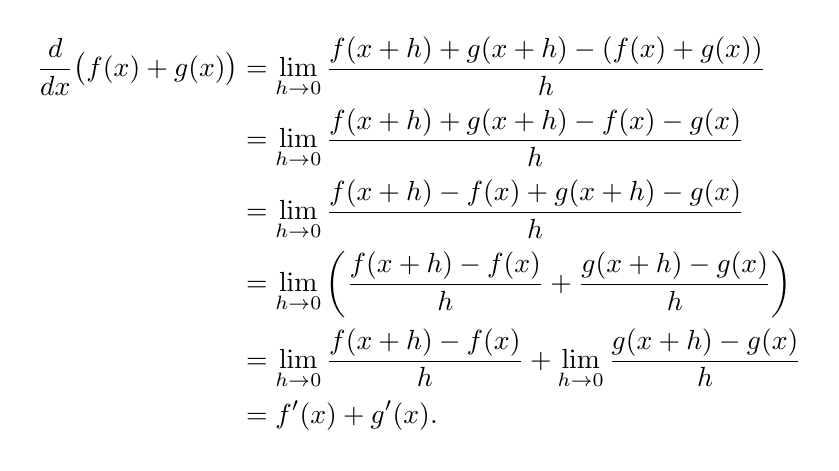
\begin{tikzpicture}
    \node at (0,0) {$\begin{aligned}
        \ddx\big(f(x)+g(x)\big) &= \lim_{ h\to 0} \frac{f(x+h)+g(x+ h) - (f(x)+g(x))}{h}  \\
        &= \lim_{ h\to 0} \frac{f(x+h)+g(x+ h) - f(x)-g(x)}{  h}  \\
        &= \lim_{ h\to 0} \frac{f(x+h)-f(x) +g(x+ h) -g(x)}{  h}  \\
        &= \lim_{ h\to 0} \left(\frac{f(x+h)-f(x)}{  h}  +\frac{g(x+ h) -g(x)}{  h}\right)  \\
        &= \lim_{ h\to 0} \frac{f(x+h)-f(x)}{  h}  +
        \lim_{ h\to 0} \frac{g(x+ h) -g(x)}{  h}  \\
        &=f'(x)+g'(x).\end{aligned}$};
    \end{tikzpicture}
\end{image}
\end{explanation}
\end{theorem}

\begin{question}
  Using different notation for the derivative can be confusing.  Which of the
  following are the same as part (a) of the Sum Rule?
  \begin{selectAll}
  	\choice[correct]{$(f(x) + g(x))' = f'(x) + g'(x)$}
	\choice[correct]{$(f(x) + g(x))' = \ddx f(x) + \ddx g(x)$}
	\choice {$\ddx f(x) + \ddx g(x) = f'(x) + g'(x)$}
	\choice {$(f'(x) + g(x))' = \ddx ( f(x) + g(x))$}
  \end{selectAll}
\end{question}


\begin{example}
  Suppose we have two functions, $f$, and $g$, and we know that $f'(2) = 6$ and $g'(2) = -3$.
  What is the slope of the tangent line to the graph $y=f(x) + g(x)$ at $x = 2$?
  \begin{explanation}
  	 The slope of the tangent line to the graph of the function $f(x) + g(x)$ at $x = 2$ is the derivative $ \eval{\ddx \left(f(x)+g(x)\right)}_{x=2}$. By the Sum Rule, this derivative is given by $f'(2) + g'(2)$.   In 
	this case, we have $f'(2) + g'(2) = \answer[given]{3}$.
  \end{explanation}
\end{example} 


We now have the tools to work some more complicated examples. 


\begin{example}
Compute:
\[
\ddx \left( x^5+\frac{1}{x}\right)
\] 
\begin{explanation}
Write with me
\begin{align*}
\ddx \left(x^5+\frac{1}{x}\right) &= \ddx x^5 + \ddx x^{-1} \\
&=\answer[given]{5x^4 - x^{-2}}.
\end{align*}
\end{explanation}
\end{example}

\begin{example}
Compute:
\[
\ddx \left(\frac{3}{\sqrt[3]{x}}-2\sqrt{x}+\frac{1}{x^7}\right)
\]
\begin{explanation}
Write with me
\begin{align*}
  \ddx &\left(\frac{3}{\sqrt[3]{x}}-2\sqrt{x}+\frac{1}{x^7}\right)\\
  &= 3\ddx x^{-1/3} -2\ddx x^{1/2}+\ddx x^{-7}\\
  &=\answer[given]{-x^{-4/3} - x^{-1/2}-7x^{-8}}.
\end{align*}
\end{explanation}
\end{example}



\end{document}
